\documentclass{article}
\usepackage{amsmath, amssymb}
\usepackage{array}
\usepackage[utf8]{inputenc}
\usepackage{graphicx}
\usepackage{subcaption}
\usepackage{enumitem}


\linespread{1.2}
\title{Assignment 2, Parallel Computing}
\author{Jinghua Feng, 661-545-981, fengj3@rpi.edu}

\begin{document}
\maketitle
In this report, only results of "test\_input\_1.txt" are shown as the execution times are more or less the same for different input files. This is due to the fact that all the test cases contain the same 262,144 hex digits.
\section{Execution at different ranks}
The plot of execution versus number of ranks are shown in Figure 1 below, which indicates that execution time is decreasing with the increase rank number. This is reasonable as the program runs faster with higher degree of parallelism. Comparing the red dash line with blue linear line, we can find that performing MPI\_Barrier operation between steps of CLA does not cause much increase of execution, with only a slight increase at rank 4 and 16. There may be two reasons behind this:
\begin{enumerate}[label=(\alph*)]
	\item Every rank conducts computation of the same number of digits, which makes their execution almost synchronized;
	\item We perform MPI\_Gather to collect data after obtaining the result of $sumi$ in each rank. MPI\_Gather is a collective communication, which can not be completed until all ranks finish their computation.
\end{enumerate}

\begin{figure}[!htb]
	\centering
	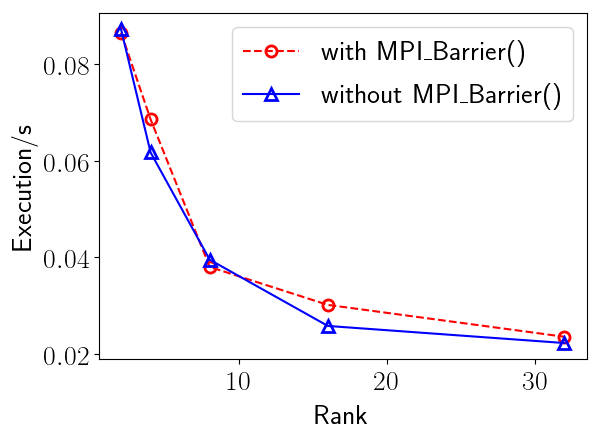
\includegraphics[scale=0.5]{../plot/exe_vs_rank.png}
	\caption{Execution time with different number of rank}
\end{figure}

\newpage
\section{Speedup relative to serial MPI CLA}
The plot of speedup relative to serial MPI CLA versus number of ranks (running time of serial MPI CLA/running time of paralleled MPI CLA) are shown in Figure 2 below, which shows that speedup increases with the growing rank number. In addition, all the speedups are greater than 1. Apparently, more ranks has higher degree of parallelism.
\begin{figure}[!htb]
	\centering   
	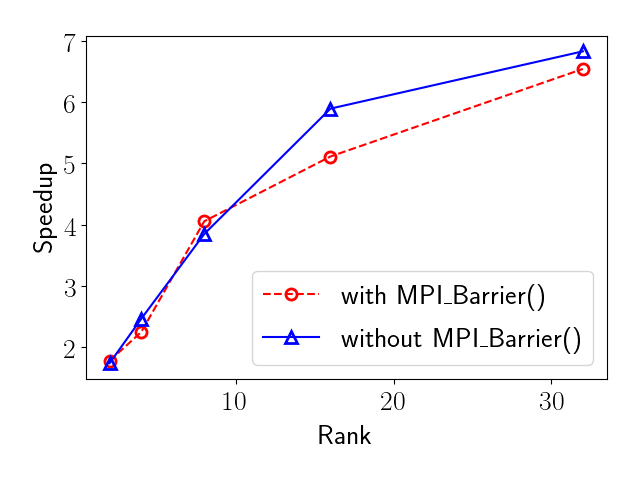
\includegraphics[scale=0.5]{../plot/speedup_rel_MPI_CLA.png}
	\caption{Speedup relative to serial MPI CLA at different number of rank}
\end{figure}

\section{Speedup relative to serial Ripple}
The plot of speedup relative to serial Ripple versus number of ranks are shown in Figure 3 below, which indicates that speedup relative to serial ripple is increasing with the growing rank number. However, the speedup is smaller than 1 for rank 2 and 4. This is because there is some overhead in paralleled MPI CLA (e.g. scattering original binary data, gathering sumi, passing supersection carry in between ranks, etc.), which may not be compensated at lower ranks. Apparently, the benefit of parallelism with rank of 8 or more can outweigh the overhead.
\begin{figure}[!htb]
	\centering
	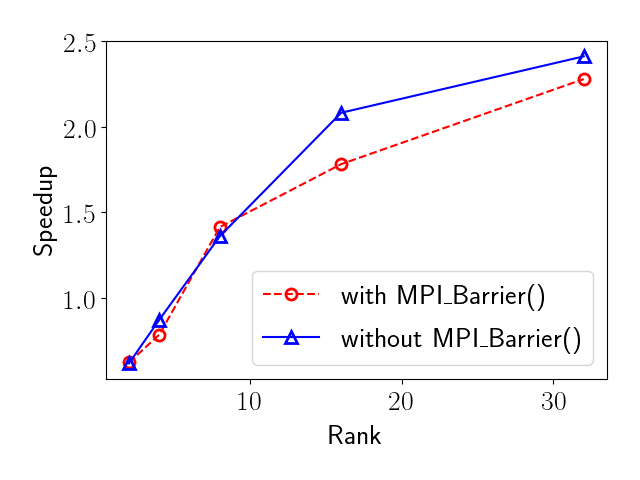
\includegraphics[scale=0.5]{../plot/speedup_rel_serial_ripple.png}
	\caption{Speedup relative to serial Ripple at different number of rank}
\end{figure}

\end{document}
